\documentclass[a4paper,landscape]{article}

\usepackage[margin=1.2cm]{geometry}
\usepackage[T1]{fontenc}
\usepackage[utf8]{inputenc}
\usepackage{lmodern}
\usepackage{amsmath,amssymb}
\usepackage{xcolor}
\usepackage{graphicx}
\usepackage{tikz}
\usetikzlibrary{arrows.meta,positioning,calc}
\usepackage[colorlinks=true,linkcolor=acousticblue,urlcolor=acousticblue,citecolor=acousticblue]{hyperref}
\hypersetup{pdfborder={0 0 0}}
\usepackage{ocgx2}
\usepackage{enumitem}

% ================= COLORS =================
\definecolor{acousticblue}{RGB}{30,60,120}
\definecolor{thermalred}{RGB}{180,0,0}
\definecolor{laserred}{RGB}{150,0,0}
\definecolor{goldau}{RGB}{200,150,0}
\definecolor{refgrey}{RGB}{120,120,120}

\tikzset{
  >=Stealth,
  bubble/.style={line width=1pt, draw=black},
  thinline/.style={line width=0.7pt},
  auxline/.style={line width=0.6pt},
}

\pagestyle{empty}
\setlength{\parindent}{0pt}

% ========= Typography knobs (tuned for Slide 7) =========
\newcommand{\SlideTitleFont}{\fontsize{28}{32}\selectfont\bfseries}
\newcommand{\ThesisFont}{\fontsize{22}{26}\selectfont}
\newcommand{\ThesisFontTight}{\fontsize{18}{21.5}\selectfont}

% ========= Toggle markers (FORCE VISIBLE) =========
% NOTE: We keep them large and colored; do not rely on link border.
\newcommand{\FigLink}[1]{\switchocg{#1}{\begingroup\setlength\fboxsep{1.2pt}\colorbox{acousticblue!15}{\textcolor{acousticblue}{\bfseries\large[fig]}}\endgroup}}
\newcommand{\EqLink}[1]{\switchocg{#1}{\begingroup\setlength\fboxsep{1.2pt}\colorbox{acousticblue!15}{\textcolor{acousticblue}{\bfseries\large[eq]}}\endgroup}}
\newcommand{\DetLink}[1]{\switchocg{#1}{\begingroup\setlength\fboxsep{1.2pt}\colorbox{acousticblue!15}{\textcolor{acousticblue}{\bfseries\large[details]}}\endgroup}}

% ========= Center overlay box (overlay ONLY; content is NOT inside \switchocg) =========
% Rationale: wrapping the whole popup content in \switchocg caused blank popups
% in Okular and unreliable behavior in Adobe. Only the [close] token is clickable.
\newcommand{\OverlayBox}[2]{%
\begin{ocg}{#1}{#1}{0}%
\begin{tikzpicture}[remember picture,overlay]%
  % soft backdrop
  \fill[white,opacity=0.88] (current page.south west) rectangle (current page.north east);
  \node[draw=black,fill=white,rounded corners=2pt,inner sep=8pt] at (current page.center)
  {\begin{minipage}{0.88\paperwidth}
     \hfill\switchocg{#1}{\begingroup\setlength\fboxsep{2pt}\colorbox{acousticblue!15}{\textcolor{acousticblue}{\bfseries\Large[close]}}\endgroup}\\[0.6em]
     #2
   \end{minipage}};
\end{tikzpicture}%
\end{ocg}%
}

\newcommand{\SlideTitle}[1]{\SlideTitleFont #1\par\vspace{0.6em}}

\begin{document}

% =====================================================
\SlideTitle{1. Cold Fusion and ``Bubble Fusion'': promises, scandals, lessons learned}
{\ThesisFont
\begin{enumerate}[label=\arabic*., leftmargin=*, itemsep=1.6em]
\item The 1989 ``cold fusion'' episode became a scientific cautionary tale: bold claims $\rightarrow$ hard verification $\rightarrow$ lasting reputational damage.
\vfill
\item In the early 2000s, ``fusion in a bottle / bubble fusion'' claims triggered a similar wave of controversy before robust replication.
\vfill
\item Key lesson: in this topic you cannot start with ``we have fusion''; you must start with \emph{verifiable quantities} and transparent diagnostics.
\end{enumerate}
}
\newpage

% =====================================================
\SlideTitle{2. Why the topic is ``toxic'' --- and my honest focus}
{\ThesisFont
\begin{enumerate}[label=\arabic*., leftmargin=*, itemsep=1.6em]
\item The community's demands are justified: independent replication, background controls, correct statistics for neutron/spectral measurements.
\vfill
\item I am not selling ``a reactor in a jar''.
\vfill
\item \textbf{Focus: not to ``prove a reaction'', but to build a testable model of temperature/energy} (and to show where the physical limitation comes from).
\end{enumerate}
}
\newpage

% =====================================================
\SlideTitle{3. Sonoluminescence: a single bubble as a micro-lab of extreme conditions \hfill \FigLink{S3photo}}
{\ThesisFont
\begin{enumerate}[label=\arabic*., leftmargin=*, itemsep=1.3em]
\item Cavitation dynamics: a bubble grows and collapses under acoustic driving $\rightarrow$ a short light flash (SBSL). \hfill \DetLink{S3def}
\vfill
\item The flash is real and reproducible; the controversy is not ``does light exist?'' but \emph{what conditions exist inside the bubble}.
\vfill
\item Core question for this talk: what is an upper bound for $T_{\max}$ at collapse, and can we shift it via an addressable energy-injection channel?
\end{enumerate}
}

\OverlayBox{S3photo}{\centering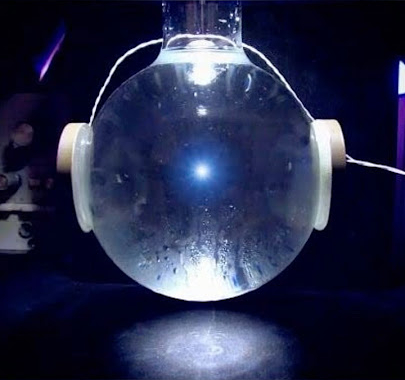
\includegraphics[height=0.70\paperheight]{oardefault.jpg}}
\OverlayBox{S3def}{\ThesisFontTight\textbf{SBSL} = \textbf{S}ingle-\textbf{B}ubble \textbf{S}ono\textbf{l}uminescence: light emission from one acoustically trapped bubble, typically with a stable periodic collapse.}

\newpage

% =====================================================
\SlideTitle{4. What careful measurements indicate: $T$ up to $\sim 2\times 10^{4}\,\mathrm{K}$, but this is often an ``effective temperature''}
{\ThesisFont
\begin{enumerate}[label=\arabic*., leftmargin=*, itemsep=1.1em]
\item Spectroscopic/SL-based estimates indicate conditions from thousands to tens of thousands of kelvin; values ``up to $2\times 10^{4}\,\mathrm{K}$'' appear in respected discussions. \hfill \DetLink{S4def}
\vfill
\item This $T$ is frequently an \emph{effective} temperature (model-dependent, radiation-weighted), which motivates a physics-based model plus cross-validation against multiple observables.
\vfill
\item Therefore the practical target is not a slogan-level number, but a constrained estimate of $T_{\max}$ with explicit assumptions and error bars.
\end{enumerate}
}

\OverlayBox{S4def}{\ThesisFontTight\textbf{SL} = \textbf{s}ono\textbf{l}uminescence in general (single-bubble or multi-bubble). ``Spectroscopic/SL-based'' here means temperature is inferred from emitted-light spectra and a chosen spectral model.}

\newpage

% =====================================================
\SlideTitle{5. Where the ``barrier'' arises: why $T_{\max}$ does not grow like an ideal adiabatic myth \hfill \FigLink{S5}}
{\ThesisFont
\begin{enumerate}[label=\arabic*., leftmargin=*, itemsep=1.3em]
\item The ideal adiabatic picture systematically overestimates heating; real physics ``eats'' energy near collapse.
\vfill
\item Barrier mechanisms: vapor effects/phase change, heat losses, chemistry/dissociation, (in extreme regimes) ionization $\rightarrow$ softening of compression and changes in effective $\gamma$.
\vfill
\item Practical implication: ``just compress harder'' may not raise $T$; an \emph{addressable, fast} energy injection near collapse is the rational route to explore.
\end{enumerate}
}

\OverlayBox{S5}{\centering
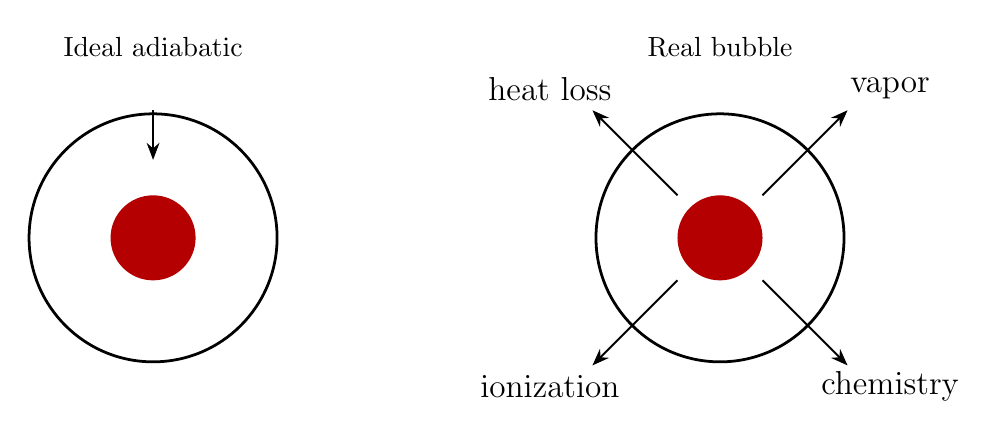
\begin{tikzpicture}[x=1cm,y=1cm,scale=0.9]
% Ideal bubble
\draw[bubble] (4,4.5) circle (1.75);
\fill[thermalred] (4,4.5) circle (0.6);
\node at (4,7.2) {Ideal adiabatic};
\draw[->,thinline] (4,6.3) -- (4,5.6);

% Real bubble
\draw[bubble] (12,4.5) circle (1.75);
\fill[thermalred] (12,4.5) circle (0.6);
\node at (12,7.2) {Real bubble};

% Leakage arrows
\draw[->,thinline] (12.6,5.1) -- (13.8,6.3);
\draw[->,thinline] (11.4,5.1) -- (10.2,6.3);
\draw[->,thinline] (12.6,3.9) -- (13.8,2.7);
\draw[->,thinline] (11.4,3.9) -- (10.2,2.7);

\node[font=\large] at (14.4,6.6) {vapor};
\node[font=\large] at (9.6,6.6) {heat loss};
\node[font=\large] at (14.4,2.4) {chemistry};
\node[font=\large] at (9.6,2.4) {ionization};
\end{tikzpicture}
}

\newpage

% =====================================================
\SlideTitle{6. Prof.\ Dr.\ Gabitov's idea: laser + AuNP as an addressable energy channel near $R_{\min}$ \hfill \FigLink{S6macro}}
{\ThesisFont
\begin{enumerate}[label=\arabic*., leftmargin=*, itemsep=0.85em]
\item Attribution: Prof.\ Dr.\ Gabitov recommended extending the model with laser pumping and Au nanoparticles (AuNP) synchronized with the final collapse stage.
\vfill
\item Physics of the channel: plasmonic absorption of AuNP $\rightarrow$ measurable absorption cross section $\sigma_{\mathrm{abs}}(\lambda,a)$ $\rightarrow$ a controlled heat/source term in the model. \hfill \FigLink{S6lspr}
\vfill
\item Carefully stated goal: estimate achievable maxima (and limits of applicability), not to claim ``fusion is already done''.
\end{enumerate}
}

\OverlayBox{S6macro}{\centering
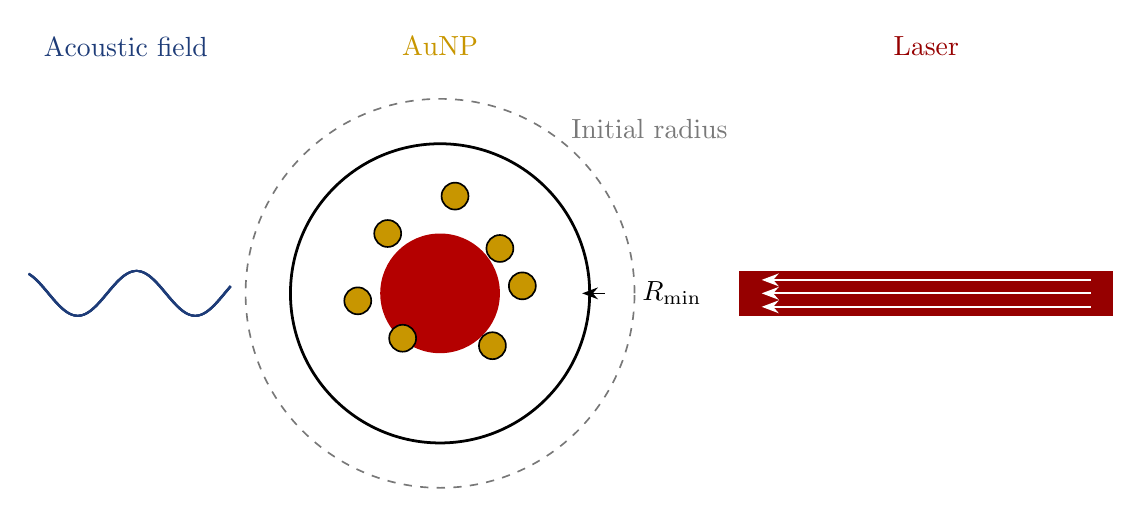
\begin{tikzpicture}[x=1cm,y=1cm,scale=0.95]
% Acoustic waves
\foreach \y in {3.5,4.2,4.9,5.6,6.3}
{
  \draw[acousticblue,thinline]
  plot[domain=0.5:3.2,samples=100]
  (\x,{4.5 + 0.3*sin(4*(\x r) + \y)});
}
\node[acousticblue,font=\normalsize] at (1.8,7.8) {Acoustic field};

% Bubble
\draw[bubble] (6,4.5) circle (2);

% Initial radius
\draw[refgrey,dashed,auxline] (6,4.5) circle (2.6);
\node[refgrey,font=\normalsize] at (8.8,6.7) {Initial radius};

% R_min label
\draw[->,auxline] (8.2,4.5) -- (7.9,4.5);
\node[font=\normalsize] at (9.1,4.5) {$R_{\min}$};

% Thermal core
\fill[thermalred] (6,4.5) circle (0.8);

% Au nanoparticles
\foreach \pos in {(5.3,5.3),(6.8,5.1),(5.5,3.9),(6.7,3.8),(6.2,5.8),(4.9,4.4),(7.1,4.6)}
{
  \fill[goldau] \pos circle (0.18);
  \draw[auxline] \pos circle (0.18);
}
\node[goldau,font=\normalsize] at (6,7.8) {AuNP};

% Laser beam body
\fill[laserred] (10,4.2) rectangle (15,4.8);

% Three stacked parallel arrows toward bubble (right -> left)
\foreach \yy in {4.32,4.50,4.68}
{
  \draw[->,white,line width=0.7pt] (14.7,\yy) -- (10.3,\yy);
}

\node[laserred,font=\normalsize] at (12.5,7.8) {Laser};
\end{tikzpicture}
}

\OverlayBox{S6lspr}{\centering
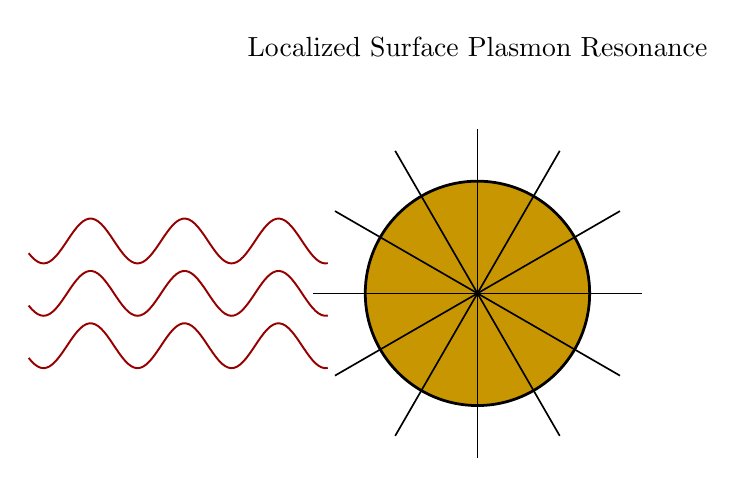
\begin{tikzpicture}[x=1cm,y=1cm,scale=0.95]
% Nanoparticle
\fill[goldau] (8,4.5) circle (1.5);
\draw[bubble] (8,4.5) circle (1.5);

% Incoming wave
\foreach \y in {3.8,4.5,5.2}
{
  \draw[laserred,thinline]
  plot[domain=2:6,samples=100]
  (\x,{ \y + 0.3*sin(5*(\x r))});
}

% Field lines
\foreach \angle in {0,30,...,330}
{
  \draw[auxline] (8,4.5) -- ++(\angle:2.2);
}
\node at (8,7.8) {Localized Surface Plasmon Resonance};
\end{tikzpicture}
}

\newpage

% =====================================================
\SlideTitle{7. My plan: modular pipeline + validation at every step \hfill \FigLink{S7pipe}}
{\ThesisFontTight
\begin{enumerate}[label=\arabic*., leftmargin=*, itemsep=0.55em]
\item Principle: not ``one huge model'', but a chain of modules where each adds \emph{one} mechanism and has a \emph{validation criterion}.
\vfill
\item Mechanics block: Rayleigh--Plesset $\rightarrow$ Keller--Miksis $\rightarrow$ produces $R(t)$, $R_{\min}$, wall velocity; validation via digitized/benchmark $R(t)$ from literature. \hfill \EqLink{S7mech}
\vfill
\item Thermodynamics + barrier block: gas energy equation with losses plus vapor/chemistry/(optional) ionization closures $\rightarrow$ produces $T(t)$ and explains why a ceiling appears. \hfill \EqLink{S7thermo}
\vfill
\item Optics + coupling block: laser$\rightarrow$AuNP absorption handled explicitly, then a coupling model AuNP$\leftrightarrow$bubble (where and when the heat is deposited). \hfill \EqLink{S7opt}
\vfill
\item Reality-control block: energy-balance checks, timescale comparisons (laser pulse duration vs collapse time), and sensitivity to uncertain parameters.
\end{enumerate}
}

\OverlayBox{S7pipe}{\centering
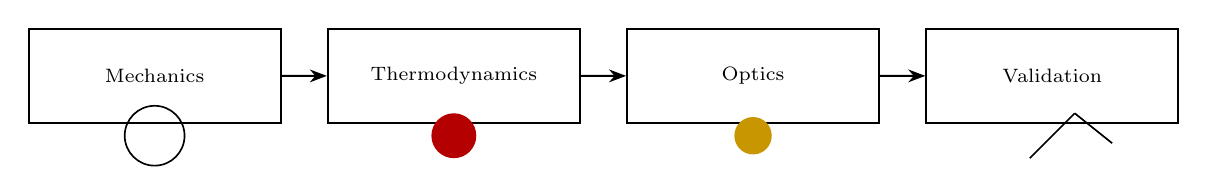
\begin{tikzpicture}[x=1cm,y=1cm,scale=0.95]
\tikzstyle{block} = [draw, rectangle, minimum width=3.2cm,
minimum height=1.2cm, line width=0.7pt, font=\scriptsize]

\node[block] (M) at (2.5,4.5) {Mechanics};
\node[block] (T) at (6.5,4.5) {Thermodynamics};
\node[block] (O) at (10.5,4.5) {Optics};
\node[block] (V) at (14.5,4.5) {Validation};

\draw[->,thinline] (M) -- (T);
\draw[->,thinline] (T) -- (O);
\draw[->,thinline] (O) -- (V);

% Minimal symbols
\draw[auxline] (2.5,3.7) circle (0.4);
\fill[thermalred] (6.5,3.7) circle (0.3);
\fill[goldau] (10.5,3.7) circle (0.25);
\draw[auxline] (14.2,3.4) -- (14.8,4.0);
\draw[auxline] (14.8,4.0) -- (15.3,3.6);
\end{tikzpicture}
}

\OverlayBox{S7mech}{\ThesisFontTight
\[
\rho\left(R\ddot R+\frac{3}{2}\dot R^2\right)
= p_{B}-p_{\infty}-\frac{2\sigma}{R}-\frac{4\mu \dot R}{R}.
\]
}

\OverlayBox{S7thermo}{\ThesisFontTight
\[
\frac{d}{dt}\left(\frac{p_B V}{\gamma-1}\right)
=-p_B\frac{dV}{dt}-\dot Q_{\mathrm{loss}}(t)+\dot Q_{\mathrm{src}}(t),
\qquad
V=\frac{4}{3}\pi R^3.
\]
}

\OverlayBox{S7opt}{\ThesisFontTight
\[
\alpha(\lambda)=4\pi a^3\frac{\varepsilon_p-\varepsilon_m}{\varepsilon_p+2\varepsilon_m},
\quad
\sigma_{\mathrm{abs}}=k\,\Im(\alpha).
\]
}

\newpage

% =====================================================
\SlideTitle{8. What you get, and what I am asking for}
{\ThesisFont
\begin{enumerate}[label=\arabic*., leftmargin=*, itemsep=1.0em]
\item You get a reproducible pipeline (code + reports) to estimate $T_{\max}$ and the limits of validity --- defensible in front of skeptics.
\vfill
\item I am asking for: academic supervision, a place in a group (internship), and/or a modest budget to bring the module chain to a publishable state.
\vfill
\item Funding framing: exploratory physics of extreme states (no ``fusion promises''), with a clean path to measurable outputs and negative-results value.
\end{enumerate}
}

\vspace{0.7em}
{\fontsize{22}{26}\selectfont \textcolor{thermalred}{\textbf{Comments and collaborations: DimitriBolt@Arizona.edu}}}

\end{document}
